\documentclass[twoside]{book}

% Packages required by doxygen
\usepackage{fixltx2e}
\usepackage{calc}
\usepackage{doxygen}
\usepackage[export]{adjustbox} % also loads graphicx
\usepackage{graphicx}
\usepackage[utf8]{inputenc}
\usepackage{makeidx}
\usepackage{multicol}
\usepackage{multirow}
\PassOptionsToPackage{warn}{textcomp}
\usepackage{textcomp}
\usepackage[nointegrals]{wasysym}
\usepackage[table]{xcolor}

% Font selection
\usepackage[T1]{fontenc}
\usepackage[scaled=.90]{helvet}
\usepackage{courier}
\usepackage{amssymb}
\usepackage{sectsty}
\renewcommand{\familydefault}{\sfdefault}
\allsectionsfont{%
  \fontseries{bc}\selectfont%
  \color{darkgray}%
}
\renewcommand{\DoxyLabelFont}{%
  \fontseries{bc}\selectfont%
  \color{darkgray}%
}
\newcommand{\+}{\discretionary{\mbox{\scriptsize$\hookleftarrow$}}{}{}}

% Page & text layout
\usepackage{geometry}
\geometry{%
  a4paper,%
  top=2.5cm,%
  bottom=2.5cm,%
  left=2.5cm,%
  right=2.5cm%
}
\tolerance=750
\hfuzz=15pt
\hbadness=750
\setlength{\emergencystretch}{15pt}
\setlength{\parindent}{0cm}
\setlength{\parskip}{3ex plus 2ex minus 2ex}
\makeatletter
\renewcommand{\paragraph}{%
  \@startsection{paragraph}{4}{0ex}{-1.0ex}{1.0ex}{%
    \normalfont\normalsize\bfseries\SS@parafont%
  }%
}
\renewcommand{\subparagraph}{%
  \@startsection{subparagraph}{5}{0ex}{-1.0ex}{1.0ex}{%
    \normalfont\normalsize\bfseries\SS@subparafont%
  }%
}
\makeatother

% Headers & footers
\usepackage{fancyhdr}
\pagestyle{fancyplain}
\fancyhead[LE]{\fancyplain{}{\bfseries\thepage}}
\fancyhead[CE]{\fancyplain{}{}}
\fancyhead[RE]{\fancyplain{}{\bfseries\leftmark}}
\fancyhead[LO]{\fancyplain{}{\bfseries\rightmark}}
\fancyhead[CO]{\fancyplain{}{}}
\fancyhead[RO]{\fancyplain{}{\bfseries\thepage}}
\fancyfoot[LE]{\fancyplain{}{}}
\fancyfoot[CE]{\fancyplain{}{}}
\fancyfoot[RE]{\fancyplain{}{\bfseries\scriptsize Generated by Doxygen }}
\fancyfoot[LO]{\fancyplain{}{\bfseries\scriptsize Generated by Doxygen }}
\fancyfoot[CO]{\fancyplain{}{}}
\fancyfoot[RO]{\fancyplain{}{}}
\renewcommand{\footrulewidth}{0.4pt}
\renewcommand{\chaptermark}[1]{%
  \markboth{#1}{}%
}
\renewcommand{\sectionmark}[1]{%
  \markright{\thesection\ #1}%
}

% Indices & bibliography
\usepackage{natbib}
\usepackage[titles]{tocloft}
\setcounter{tocdepth}{3}
\setcounter{secnumdepth}{5}
\makeindex

% Hyperlinks (required, but should be loaded last)
\usepackage{ifpdf}
\ifpdf
  \usepackage[pdftex,pagebackref=true]{hyperref}
\else
  \usepackage[ps2pdf,pagebackref=true]{hyperref}
\fi
\hypersetup{%
  colorlinks=true,%
  linkcolor=blue,%
  citecolor=blue,%
  unicode%
}

% Custom commands
\newcommand{\clearemptydoublepage}{%
  \newpage{\pagestyle{empty}\cleardoublepage}%
}

\usepackage{caption}
\captionsetup{labelsep=space,justification=centering,font={bf},singlelinecheck=off,skip=4pt,position=top}

%===== C O N T E N T S =====

\begin{document}

% Titlepage & ToC
\hypersetup{pageanchor=false,
             bookmarksnumbered=true,
             pdfencoding=unicode
            }
\pagenumbering{alph}
\begin{titlepage}
\vspace*{7cm}
\begin{center}%
{\Large Documentation Cpp \\[1ex]\large 1.\+0 }\\
\vspace*{1cm}
{\large Generated by Doxygen 1.8.13}\\
\end{center}
\end{titlepage}
\clearemptydoublepage
\pagenumbering{roman}
\tableofcontents
\clearemptydoublepage
\pagenumbering{arabic}
\hypersetup{pageanchor=true}

%--- Begin generated contents ---
\chapter{Hierarchical Index}
\section{Class Hierarchy}
This inheritance list is sorted roughly, but not completely, alphabetically\+:\begin{DoxyCompactList}
\item \contentsline{section}{Deserializer}{\pageref{struct_deserializer}}{}
\item Print\begin{DoxyCompactList}
\item \contentsline{section}{ostream}{\pageref{classostream}}{}
\end{DoxyCompactList}
\item \contentsline{section}{Serializer}{\pageref{struct_serializer}}{}
\item \contentsline{section}{Serial\+Talks}{\pageref{class_serial_talks}}{}
\end{DoxyCompactList}

\chapter{Class Index}
\section{Class List}
Here are the classes, structs, unions and interfaces with brief descriptions\+:\begin{DoxyCompactList}
\item\contentsline{section}{\hyperlink{struct_deserializer}{Deserializer} \\*Objet destiné à extraire des variables d\textquotesingle{}un flux en octet }{\pageref{struct_deserializer}}{}
\item\contentsline{section}{\hyperlink{classostream}{ostream} }{\pageref{classostream}}{}
\item\contentsline{section}{\hyperlink{struct_serializer}{Serializer} \\*Objet destiné à creer un flux de sortie pour les programme cpp }{\pageref{struct_serializer}}{}
\item\contentsline{section}{\hyperlink{class_serial_talks}{Serial\+Talks} \\*Object de communication serial avec un ordinateur }{\pageref{class_serial_talks}}{}
\end{DoxyCompactList}

\chapter{File Index}
\section{File List}
Here is a list of all files with brief descriptions\+:\begin{DoxyCompactList}
\item\contentsline{section}{source\+\_\+code/\hyperlink{_serial_talks_8h}{Serial\+Talks.\+h} }{\pageref{_serial_talks_8h}}{}
\item\contentsline{section}{source\+\_\+code/\hyperlink{serialutils_8h}{serialutils.\+h} }{\pageref{serialutils_8h}}{}
\end{DoxyCompactList}

\chapter{Class Documentation}
\hypertarget{struct_deserializer}{}\section{Deserializer Struct Reference}
\label{struct_deserializer}\index{Deserializer@{Deserializer}}


Objet destiné à extraire des variables d\textquotesingle{}un flux en octet.  




{\ttfamily \#include $<$serialutils.\+h$>$}

\subsection*{Public Member Functions}
\begin{DoxyCompactItemize}
\item 
\hyperlink{struct_deserializer_ae6463833d115113e2d7ed91c79d0c988}{Deserializer} (\hyperlink{serialutils_8h_a0c8186d9b9b7880309c27230bbb5e69d}{byte} \hyperlink{struct_deserializer_a37f4bae0d8a61c6c556ba3e90a10f0c4}{buffer}\mbox{[}$\,$\mbox{]})
\begin{DoxyCompactList}\small\item\em Constructeur de \hyperlink{struct_deserializer}{Deserializer}. \end{DoxyCompactList}\item 
{\footnotesize template$<$typename T $>$ }\\\hyperlink{struct_deserializer}{Deserializer} \& \hyperlink{struct_deserializer_acda0fe1ee62c4f5de3d70104a20bc41a}{operator$>$$>$} (T \&object)
\begin{DoxyCompactList}\small\item\em Operateur de décalage, a utilisé pour extraire les variables du buffer. \end{DoxyCompactList}\item 
\hyperlink{struct_deserializer}{Deserializer} \& \hyperlink{struct_deserializer_aef72a346514298e1e71e69e9aef3b96f}{operator$>$$>$} (char $\ast$string)
\begin{DoxyCompactList}\small\item\em Operateur de décalage, a utilisé pour remplir le buffer uniquement pour les variables de type char. \end{DoxyCompactList}\item 
{\footnotesize template$<$typename T $>$ }\\T \hyperlink{struct_deserializer_af93dc898d561ad0b1d8b86ddf49053ca}{read} ()
\begin{DoxyCompactList}\small\item\em Methode interne pour convertir les octets du buffer en données exploitables. \end{DoxyCompactList}\item 
{\footnotesize template$<$$>$ }\\\hyperlink{serialutils_8h_afbeda3fd1bdc8c37d01bdf9f5c8274ff}{String} \hyperlink{struct_deserializer_aefa095423e11239219f8a472547a6d22}{read} ()
\end{DoxyCompactItemize}
\subsection*{Public Attributes}
\begin{DoxyCompactItemize}
\item 
\hyperlink{serialutils_8h_a0c8186d9b9b7880309c27230bbb5e69d}{byte} $\ast$ \hyperlink{struct_deserializer_a37f4bae0d8a61c6c556ba3e90a10f0c4}{buffer}
\end{DoxyCompactItemize}


\subsection{Detailed Description}
Objet destiné à extraire des variables d\textquotesingle{}un flux en octet. 

\hyperlink{struct_deserializer}{Deserializer} permet d\textquotesingle{}extraire d\textquotesingle{}un buffer des variables. Cela permet une utilisation plus simple de \hyperlink{class_serial_talks}{Serial\+Talks}. Voir l\textquotesingle{}utilisation dans la doc python. Attention a bien extraire les variables dans le bonne ordre pour éviter les problèmes d\textquotesingle{}encodage et autres. 

\subsection{Constructor \& Destructor Documentation}
\mbox{\Hypertarget{struct_deserializer_ae6463833d115113e2d7ed91c79d0c988}\label{struct_deserializer_ae6463833d115113e2d7ed91c79d0c988}} 
\index{Deserializer@{Deserializer}!Deserializer@{Deserializer}}
\index{Deserializer@{Deserializer}!Deserializer@{Deserializer}}
\subsubsection{\texorpdfstring{Deserializer()}{Deserializer()}}
{\footnotesize\ttfamily Deserializer\+::\+Deserializer (\begin{DoxyParamCaption}\item[{\hyperlink{serialutils_8h_a0c8186d9b9b7880309c27230bbb5e69d}{byte}}]{buffer\mbox{[}$\,$\mbox{]} }\end{DoxyParamCaption})\hspace{0.3cm}{\ttfamily [inline]}}



Constructeur de \hyperlink{struct_deserializer}{Deserializer}. 


\begin{DoxyParams}{Parameters}
{\em buffer} & pointeur du buffer à utiliser. \\
\hline
\end{DoxyParams}


\subsection{Member Function Documentation}
\mbox{\Hypertarget{struct_deserializer_acda0fe1ee62c4f5de3d70104a20bc41a}\label{struct_deserializer_acda0fe1ee62c4f5de3d70104a20bc41a}} 
\index{Deserializer@{Deserializer}!operator$>$$>$@{operator$>$$>$}}
\index{operator$>$$>$@{operator$>$$>$}!Deserializer@{Deserializer}}
\subsubsection{\texorpdfstring{operator$>$$>$()}{operator>>()}\hspace{0.1cm}{\footnotesize\ttfamily [1/2]}}
{\footnotesize\ttfamily template$<$typename T $>$ \\
\hyperlink{struct_deserializer}{Deserializer}\& Deserializer\+::operator$>$$>$ (\begin{DoxyParamCaption}\item[{T \&}]{object }\end{DoxyParamCaption})\hspace{0.3cm}{\ttfamily [inline]}}



Operateur de décalage, a utilisé pour extraire les variables du buffer. 


\begin{DoxyParams}{Parameters}
{\em object} & Object à complêter avec le buffer. Attention le type de la variable est pris en compte dans la conversion octect -\/$>$ var\\
\hline
\end{DoxyParams}
\begin{DoxyReturn}{Returns}
Retourne le pointeur du deserializer pour une utilisation plus simple. 
\end{DoxyReturn}
\mbox{\Hypertarget{struct_deserializer_aef72a346514298e1e71e69e9aef3b96f}\label{struct_deserializer_aef72a346514298e1e71e69e9aef3b96f}} 
\index{Deserializer@{Deserializer}!operator$>$$>$@{operator$>$$>$}}
\index{operator$>$$>$@{operator$>$$>$}!Deserializer@{Deserializer}}
\subsubsection{\texorpdfstring{operator$>$$>$()}{operator>>()}\hspace{0.1cm}{\footnotesize\ttfamily [2/2]}}
{\footnotesize\ttfamily \hyperlink{struct_deserializer}{Deserializer}\& Deserializer\+::operator$>$$>$ (\begin{DoxyParamCaption}\item[{char $\ast$}]{string }\end{DoxyParamCaption})\hspace{0.3cm}{\ttfamily [inline]}}



Operateur de décalage, a utilisé pour remplir le buffer uniquement pour les variables de type char. 


\begin{DoxyParams}{Parameters}
{\em object} & Object a renvoyer dans le buffer pour transmission.\\
\hline
\end{DoxyParams}
\begin{DoxyReturn}{Returns}
Retourne le pointeur du serializer pour une utilisation plus simple 
\end{DoxyReturn}
\mbox{\Hypertarget{struct_deserializer_af93dc898d561ad0b1d8b86ddf49053ca}\label{struct_deserializer_af93dc898d561ad0b1d8b86ddf49053ca}} 
\index{Deserializer@{Deserializer}!read@{read}}
\index{read@{read}!Deserializer@{Deserializer}}
\subsubsection{\texorpdfstring{read()}{read()}\hspace{0.1cm}{\footnotesize\ttfamily [1/2]}}
{\footnotesize\ttfamily template$<$typename T $>$ \\
T Deserializer\+::read (\begin{DoxyParamCaption}{ }\end{DoxyParamCaption})\hspace{0.3cm}{\ttfamily [inline]}}



Methode interne pour convertir les octets du buffer en données exploitables. 

\begin{DoxyReturn}{Returns}
Retourne la valeur extraite du buffer. 
\end{DoxyReturn}
\mbox{\Hypertarget{struct_deserializer_aefa095423e11239219f8a472547a6d22}\label{struct_deserializer_aefa095423e11239219f8a472547a6d22}} 
\index{Deserializer@{Deserializer}!read@{read}}
\index{read@{read}!Deserializer@{Deserializer}}
\subsubsection{\texorpdfstring{read()}{read()}\hspace{0.1cm}{\footnotesize\ttfamily [2/2]}}
{\footnotesize\ttfamily template$<$$>$ \\
\hyperlink{serialutils_8h_afbeda3fd1bdc8c37d01bdf9f5c8274ff}{String} Deserializer\+::read (\begin{DoxyParamCaption}{ }\end{DoxyParamCaption})\hspace{0.3cm}{\ttfamily [inline]}}



\subsection{Member Data Documentation}
\mbox{\Hypertarget{struct_deserializer_a37f4bae0d8a61c6c556ba3e90a10f0c4}\label{struct_deserializer_a37f4bae0d8a61c6c556ba3e90a10f0c4}} 
\index{Deserializer@{Deserializer}!buffer@{buffer}}
\index{buffer@{buffer}!Deserializer@{Deserializer}}
\subsubsection{\texorpdfstring{buffer}{buffer}}
{\footnotesize\ttfamily \hyperlink{serialutils_8h_a0c8186d9b9b7880309c27230bbb5e69d}{byte}$\ast$ Deserializer\+::buffer}

pointer vers le buffer à vider 

The documentation for this struct was generated from the following file\+:\begin{DoxyCompactItemize}
\item 
source\+\_\+code/\hyperlink{serialutils_8h}{serialutils.\+h}\end{DoxyCompactItemize}

\hypertarget{classostream}{}\section{ostream Class Reference}
\label{classostream}\index{ostream@{ostream}}


{\ttfamily \#include $<$Serial\+Talks.\+h$>$}

Inheritance diagram for ostream\+:\begin{figure}[H]
\begin{center}
\leavevmode
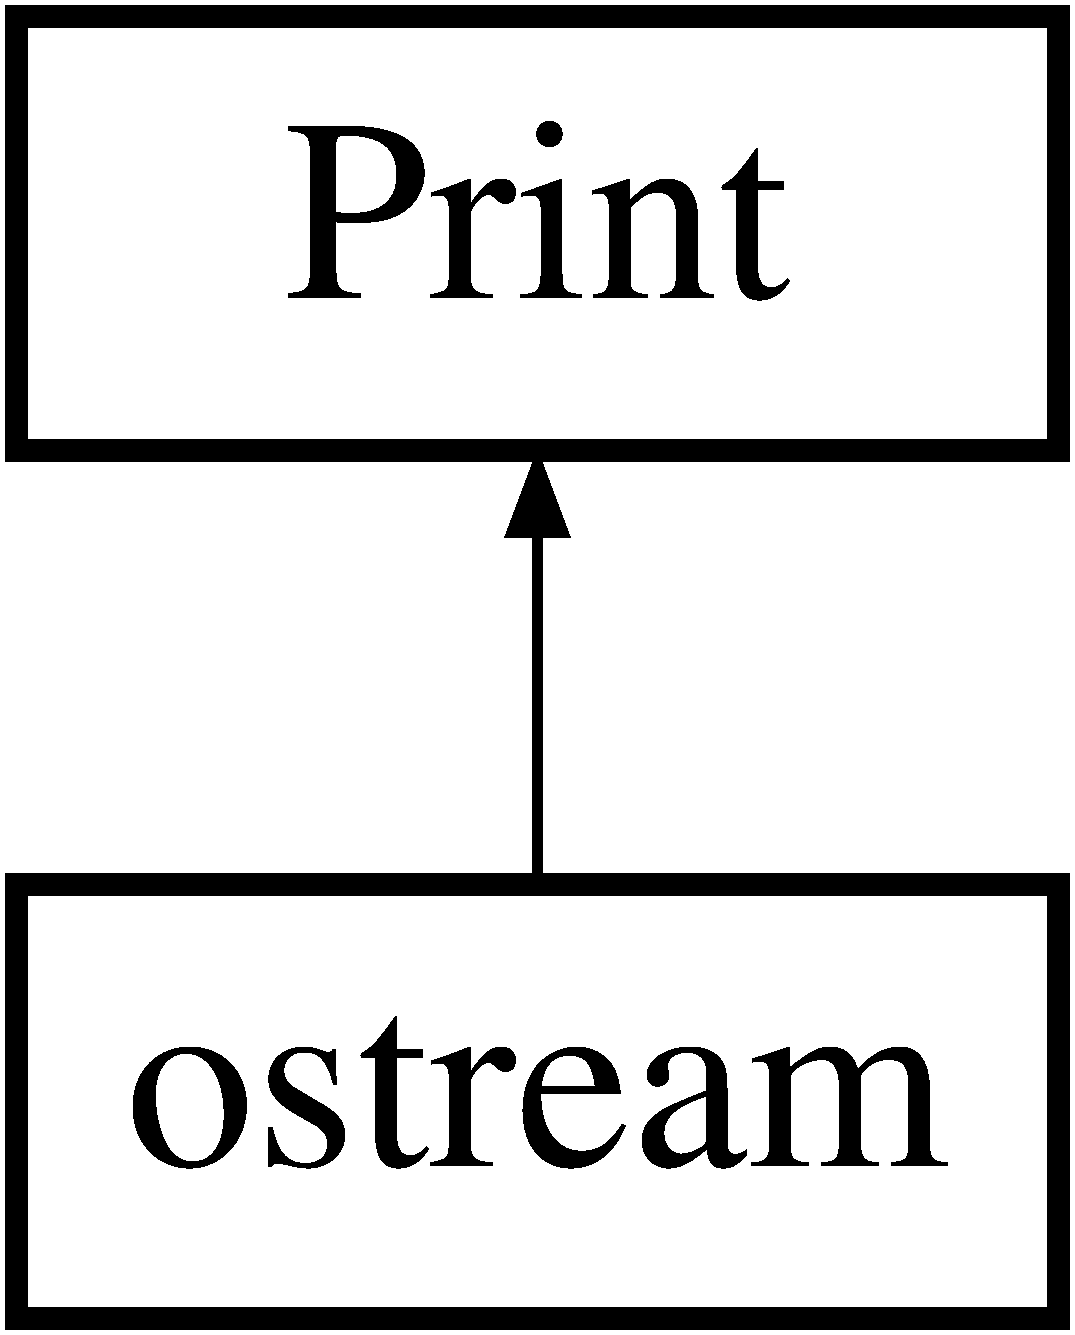
\includegraphics[height=2.000000cm]{classostream}
\end{center}
\end{figure}
\subsection*{Public Member Functions}
\begin{DoxyCompactItemize}
\item 
virtual size\+\_\+t \hyperlink{classostream_a6f8b701c1cb3f122bf13074034520295}{write} (uint8\+\_\+t)
\item 
virtual size\+\_\+t \hyperlink{classostream_a3beab2da985550ca8ba66b4a77a410fb}{write} (const uint8\+\_\+t $\ast$buffer, size\+\_\+t size)
\item 
{\footnotesize template$<$typename T $>$ }\\\hyperlink{classostream}{ostream} \& \hyperlink{classostream_a9cb0d22f302c0f6617759ec2865f7704}{operator$<$$<$} (const T \&object)
\end{DoxyCompactItemize}
\subsection*{Protected Member Functions}
\begin{DoxyCompactItemize}
\item 
void \hyperlink{classostream_a55897fe17941a52bd6b192fc71282bc2}{begin} (\hyperlink{class_serial_talks}{Serial\+Talks} \&parent, long retcode)
\end{DoxyCompactItemize}
\subsection*{Protected Attributes}
\begin{DoxyCompactItemize}
\item 
\hyperlink{class_serial_talks}{Serial\+Talks} $\ast$ \hyperlink{classostream_ae7a12b9eca5c965ccaf44e09a63c4395}{m\+\_\+parent}
\item 
long \hyperlink{classostream_a00f9816ccfffe3c50d00726be18270a3}{m\+\_\+retcode}
\end{DoxyCompactItemize}
\subsection*{Friends}
\begin{DoxyCompactItemize}
\item 
class \hyperlink{classostream_a4cd752c675c62b44d1424308b66cf98c}{Serial\+Talks}
\end{DoxyCompactItemize}


\subsection{Member Function Documentation}
\mbox{\Hypertarget{classostream_a55897fe17941a52bd6b192fc71282bc2}\label{classostream_a55897fe17941a52bd6b192fc71282bc2}} 
\index{ostream@{ostream}!begin@{begin}}
\index{begin@{begin}!ostream@{ostream}}
\subsubsection{\texorpdfstring{begin()}{begin()}}
{\footnotesize\ttfamily void ostream\+::begin (\begin{DoxyParamCaption}\item[{\hyperlink{class_serial_talks}{Serial\+Talks} \&}]{parent,  }\item[{long}]{retcode }\end{DoxyParamCaption})\hspace{0.3cm}{\ttfamily [protected]}}

\mbox{\Hypertarget{classostream_a9cb0d22f302c0f6617759ec2865f7704}\label{classostream_a9cb0d22f302c0f6617759ec2865f7704}} 
\index{ostream@{ostream}!operator$<$$<$@{operator$<$$<$}}
\index{operator$<$$<$@{operator$<$$<$}!ostream@{ostream}}
\subsubsection{\texorpdfstring{operator$<$$<$()}{operator<<()}}
{\footnotesize\ttfamily template$<$typename T $>$ \\
\hyperlink{classostream}{ostream}\& ostream\+::operator$<$$<$ (\begin{DoxyParamCaption}\item[{const T \&}]{object }\end{DoxyParamCaption})\hspace{0.3cm}{\ttfamily [inline]}}

\mbox{\Hypertarget{classostream_a6f8b701c1cb3f122bf13074034520295}\label{classostream_a6f8b701c1cb3f122bf13074034520295}} 
\index{ostream@{ostream}!write@{write}}
\index{write@{write}!ostream@{ostream}}
\subsubsection{\texorpdfstring{write()}{write()}\hspace{0.1cm}{\footnotesize\ttfamily [1/2]}}
{\footnotesize\ttfamily virtual size\+\_\+t ostream\+::write (\begin{DoxyParamCaption}\item[{uint8\+\_\+t}]{ }\end{DoxyParamCaption})\hspace{0.3cm}{\ttfamily [virtual]}}

\mbox{\Hypertarget{classostream_a3beab2da985550ca8ba66b4a77a410fb}\label{classostream_a3beab2da985550ca8ba66b4a77a410fb}} 
\index{ostream@{ostream}!write@{write}}
\index{write@{write}!ostream@{ostream}}
\subsubsection{\texorpdfstring{write()}{write()}\hspace{0.1cm}{\footnotesize\ttfamily [2/2]}}
{\footnotesize\ttfamily virtual size\+\_\+t ostream\+::write (\begin{DoxyParamCaption}\item[{const uint8\+\_\+t $\ast$}]{buffer,  }\item[{size\+\_\+t}]{size }\end{DoxyParamCaption})\hspace{0.3cm}{\ttfamily [virtual]}}



\subsection{Friends And Related Function Documentation}
\mbox{\Hypertarget{classostream_a4cd752c675c62b44d1424308b66cf98c}\label{classostream_a4cd752c675c62b44d1424308b66cf98c}} 
\index{ostream@{ostream}!Serial\+Talks@{Serial\+Talks}}
\index{Serial\+Talks@{Serial\+Talks}!ostream@{ostream}}
\subsubsection{\texorpdfstring{Serial\+Talks}{SerialTalks}}
{\footnotesize\ttfamily friend class \hyperlink{class_serial_talks}{Serial\+Talks}\hspace{0.3cm}{\ttfamily [friend]}}



\subsection{Member Data Documentation}
\mbox{\Hypertarget{classostream_ae7a12b9eca5c965ccaf44e09a63c4395}\label{classostream_ae7a12b9eca5c965ccaf44e09a63c4395}} 
\index{ostream@{ostream}!m\+\_\+parent@{m\+\_\+parent}}
\index{m\+\_\+parent@{m\+\_\+parent}!ostream@{ostream}}
\subsubsection{\texorpdfstring{m\+\_\+parent}{m\_parent}}
{\footnotesize\ttfamily \hyperlink{class_serial_talks}{Serial\+Talks}$\ast$ ostream\+::m\+\_\+parent\hspace{0.3cm}{\ttfamily [protected]}}

\mbox{\Hypertarget{classostream_a00f9816ccfffe3c50d00726be18270a3}\label{classostream_a00f9816ccfffe3c50d00726be18270a3}} 
\index{ostream@{ostream}!m\+\_\+retcode@{m\+\_\+retcode}}
\index{m\+\_\+retcode@{m\+\_\+retcode}!ostream@{ostream}}
\subsubsection{\texorpdfstring{m\+\_\+retcode}{m\_retcode}}
{\footnotesize\ttfamily long ostream\+::m\+\_\+retcode\hspace{0.3cm}{\ttfamily [protected]}}



The documentation for this class was generated from the following file\+:\begin{DoxyCompactItemize}
\item 
source\+\_\+code/\hyperlink{_serial_talks_8h}{Serial\+Talks.\+h}\end{DoxyCompactItemize}

\hypertarget{struct_serializer}{}\section{Serializer Struct Reference}
\label{struct_serializer}\index{Serializer@{Serializer}}


Objet destiné à creer un flux de sortie pour les programme cpp.  




{\ttfamily \#include $<$serialutils.\+h$>$}

\subsection*{Public Member Functions}
\begin{DoxyCompactItemize}
\item 
\hyperlink{struct_serializer_aff15a74ed17c990475261e4d1319ca7a}{Serializer} (\hyperlink{serialutils_8h_a0c8186d9b9b7880309c27230bbb5e69d}{byte} \hyperlink{struct_serializer_a2c1edbc67c09dcfffe63194038fd9566}{buffer}\mbox{[}$\,$\mbox{]})
\begin{DoxyCompactList}\small\item\em Constructeur de \hyperlink{struct_serializer}{Serializer}. \end{DoxyCompactList}\item 
{\footnotesize template$<$typename T $>$ }\\\hyperlink{struct_serializer}{Serializer} \& \hyperlink{struct_serializer_a984119e4cc29ca38db4c193b70efe211}{operator$<$$<$} (const T \&object)
\begin{DoxyCompactList}\small\item\em Operateur de décalage, a utilisé pour remplir le buffer. \end{DoxyCompactList}\item 
{\footnotesize template$<$typename T $>$ }\\void \hyperlink{struct_serializer_a1ee0f154ba82fc4cfb1bf596debc69d4}{write} (const T \&object)
\begin{DoxyCompactList}\small\item\em Methode pour une utilisation interne qui permet d\textquotesingle{}écrire sur le buffer après conversion en octets. \end{DoxyCompactList}\item 
void \hyperlink{struct_serializer_ac0afd6edf14f126f8c7f95d670d83d0b}{write} (const char $\ast$string)
\begin{DoxyCompactList}\small\item\em Methode pour une utilisation interne qui permet d\textquotesingle{}écrire sur le buffer après conversion en octets. \end{DoxyCompactList}\item 
{\footnotesize template$<$$>$ }\\void \hyperlink{struct_serializer_a1538c2a1dbc7eca145e370c1a1619d59}{write} (const \hyperlink{serialutils_8h_afbeda3fd1bdc8c37d01bdf9f5c8274ff}{String} \&string)
\end{DoxyCompactItemize}
\subsection*{Public Attributes}
\begin{DoxyCompactItemize}
\item 
\hyperlink{serialutils_8h_a0c8186d9b9b7880309c27230bbb5e69d}{byte} $\ast$ \hyperlink{struct_serializer_a2c1edbc67c09dcfffe63194038fd9566}{buffer}
\end{DoxyCompactItemize}


\subsection{Detailed Description}
Objet destiné à creer un flux de sortie pour les programme cpp. 

\hyperlink{struct_serializer}{Serializer} permet de remplir un buffer en octet à l\textquotesingle{}aide de variable de tous type. Cela permet une utilisation plus simple de \hyperlink{class_serial_talks}{Serial\+Talks}. Voir l\textquotesingle{}utilisation dans la doc python. 

\subsection{Constructor \& Destructor Documentation}
\mbox{\Hypertarget{struct_serializer_aff15a74ed17c990475261e4d1319ca7a}\label{struct_serializer_aff15a74ed17c990475261e4d1319ca7a}} 
\index{Serializer@{Serializer}!Serializer@{Serializer}}
\index{Serializer@{Serializer}!Serializer@{Serializer}}
\subsubsection{\texorpdfstring{Serializer()}{Serializer()}}
{\footnotesize\ttfamily Serializer\+::\+Serializer (\begin{DoxyParamCaption}\item[{\hyperlink{serialutils_8h_a0c8186d9b9b7880309c27230bbb5e69d}{byte}}]{buffer\mbox{[}$\,$\mbox{]} }\end{DoxyParamCaption})\hspace{0.3cm}{\ttfamily [inline]}}



Constructeur de \hyperlink{struct_serializer}{Serializer}. 


\begin{DoxyParams}{Parameters}
{\em buffer} & pointeur du buffer. \\
\hline
\end{DoxyParams}


\subsection{Member Function Documentation}
\mbox{\Hypertarget{struct_serializer_a984119e4cc29ca38db4c193b70efe211}\label{struct_serializer_a984119e4cc29ca38db4c193b70efe211}} 
\index{Serializer@{Serializer}!operator$<$$<$@{operator$<$$<$}}
\index{operator$<$$<$@{operator$<$$<$}!Serializer@{Serializer}}
\subsubsection{\texorpdfstring{operator$<$$<$()}{operator<<()}}
{\footnotesize\ttfamily template$<$typename T $>$ \\
\hyperlink{struct_serializer}{Serializer}\& Serializer\+::operator$<$$<$ (\begin{DoxyParamCaption}\item[{const T \&}]{object }\end{DoxyParamCaption})\hspace{0.3cm}{\ttfamily [inline]}}



Operateur de décalage, a utilisé pour remplir le buffer. 


\begin{DoxyParams}{Parameters}
{\em object} & Object a renvoyer dans le buffer pour transmission.\\
\hline
\end{DoxyParams}
\begin{DoxyReturn}{Returns}
Retourne le pointeur du serializer pour une utilisation plus simple 
\end{DoxyReturn}
\mbox{\Hypertarget{struct_serializer_a1ee0f154ba82fc4cfb1bf596debc69d4}\label{struct_serializer_a1ee0f154ba82fc4cfb1bf596debc69d4}} 
\index{Serializer@{Serializer}!write@{write}}
\index{write@{write}!Serializer@{Serializer}}
\subsubsection{\texorpdfstring{write()}{write()}\hspace{0.1cm}{\footnotesize\ttfamily [1/3]}}
{\footnotesize\ttfamily template$<$typename T $>$ \\
void Serializer\+::write (\begin{DoxyParamCaption}\item[{const T \&}]{object }\end{DoxyParamCaption})\hspace{0.3cm}{\ttfamily [inline]}}



Methode pour une utilisation interne qui permet d\textquotesingle{}écrire sur le buffer après conversion en octets. 


\begin{DoxyParams}{Parameters}
{\em object} & Object a renvoyer dans le buffer pour ecriture. \\
\hline
\end{DoxyParams}
\mbox{\Hypertarget{struct_serializer_ac0afd6edf14f126f8c7f95d670d83d0b}\label{struct_serializer_ac0afd6edf14f126f8c7f95d670d83d0b}} 
\index{Serializer@{Serializer}!write@{write}}
\index{write@{write}!Serializer@{Serializer}}
\subsubsection{\texorpdfstring{write()}{write()}\hspace{0.1cm}{\footnotesize\ttfamily [2/3]}}
{\footnotesize\ttfamily void Serializer\+::write (\begin{DoxyParamCaption}\item[{const char $\ast$}]{string }\end{DoxyParamCaption})\hspace{0.3cm}{\ttfamily [inline]}}



Methode pour une utilisation interne qui permet d\textquotesingle{}écrire sur le buffer après conversion en octets. 


\begin{DoxyParams}{Parameters}
{\em object} & Object (sous la forme d\textquotesingle{}un char) a renvoyer dans le buffer pour ecriture. \\
\hline
\end{DoxyParams}
\mbox{\Hypertarget{struct_serializer_a1538c2a1dbc7eca145e370c1a1619d59}\label{struct_serializer_a1538c2a1dbc7eca145e370c1a1619d59}} 
\index{Serializer@{Serializer}!write@{write}}
\index{write@{write}!Serializer@{Serializer}}
\subsubsection{\texorpdfstring{write()}{write()}\hspace{0.1cm}{\footnotesize\ttfamily [3/3]}}
{\footnotesize\ttfamily template$<$$>$ \\
void Serializer\+::write (\begin{DoxyParamCaption}\item[{const \hyperlink{serialutils_8h_afbeda3fd1bdc8c37d01bdf9f5c8274ff}{String} \&}]{string }\end{DoxyParamCaption})\hspace{0.3cm}{\ttfamily [inline]}}



\subsection{Member Data Documentation}
\mbox{\Hypertarget{struct_serializer_a2c1edbc67c09dcfffe63194038fd9566}\label{struct_serializer_a2c1edbc67c09dcfffe63194038fd9566}} 
\index{Serializer@{Serializer}!buffer@{buffer}}
\index{buffer@{buffer}!Serializer@{Serializer}}
\subsubsection{\texorpdfstring{buffer}{buffer}}
{\footnotesize\ttfamily \hyperlink{serialutils_8h_a0c8186d9b9b7880309c27230bbb5e69d}{byte}$\ast$ Serializer\+::buffer}

pointer vers le buffer à complêter 

The documentation for this struct was generated from the following file\+:\begin{DoxyCompactItemize}
\item 
source\+\_\+code/\hyperlink{serialutils_8h}{serialutils.\+h}\end{DoxyCompactItemize}

\hypertarget{class_serial_talks}{}\section{Serial\+Talks Class Reference}
\label{class_serial_talks}\index{Serial\+Talks@{Serial\+Talks}}


Object de communication serial avec un ordinateur.  




{\ttfamily \#include $<$Serial\+Talks.\+h$>$}

\subsection*{Public Types}
\begin{DoxyCompactItemize}
\item 
typedef void($\ast$ \hyperlink{class_serial_talks_a35ccf86c63ad45fb719e81b0c8db2f13}{Instruction}) (\hyperlink{class_serial_talks}{Serial\+Talks} \&inst, \hyperlink{struct_deserializer}{Deserializer} \&input, \hyperlink{struct_serializer}{Serializer} \&output)
\end{DoxyCompactItemize}
\subsection*{Public Member Functions}
\begin{DoxyCompactItemize}
\item 
void \hyperlink{class_serial_talks_ad66e8c5cd4d3ae3e63f70884dba3ce12}{begin} (Stream \&stream)
\item 
void \hyperlink{class_serial_talks_a484c56fb8d8619a58435a001dca6f0ba}{bind} (\hyperlink{serialutils_8h_a0c8186d9b9b7880309c27230bbb5e69d}{byte} opcode, \hyperlink{class_serial_talks_a35ccf86c63ad45fb719e81b0c8db2f13}{Instruction} instruction)
\item 
bool \hyperlink{class_serial_talks_a31aac8c9995468cf9b1308264bc077ae}{execinstruction} (\hyperlink{serialutils_8h_a0c8186d9b9b7880309c27230bbb5e69d}{byte} $\ast$input\+Buffer)
\item 
bool \hyperlink{class_serial_talks_a9bd8eaff71cfcf33f489e86d3326435c}{execute} ()
\item 
bool \hyperlink{class_serial_talks_a02d73ff9cbb4c44e2e9ba36f97714c9d}{is\+Connected} () const
\item 
bool \hyperlink{class_serial_talks_a1cf3e5668f7a1d1cd1296535ef011528}{wait\+Until\+Connected} (float timeout=-\/1)
\item 
bool \hyperlink{class_serial_talks_a61f0840f12d804ea107ebb98abdc5964}{get\+U\+U\+ID} (char $\ast$uuid)
\item 
void \hyperlink{class_serial_talks_a66e896e6d974c4e4eb9ed890b15c38c1}{set\+U\+U\+ID} (const char $\ast$uuid)
\end{DoxyCompactItemize}
\subsection*{Static Public Member Functions}
\begin{DoxyCompactItemize}
\item 
static void \hyperlink{class_serial_talks_a08807e3d40b70042f9b88504216245e0}{generate\+Random\+U\+U\+ID} (char $\ast$uuid, int length)
\end{DoxyCompactItemize}
\subsection*{Public Attributes}
\begin{DoxyCompactItemize}
\item 
\hyperlink{classostream}{ostream} \hyperlink{class_serial_talks_adcce1950be020551b2acfac6c912bbb8}{out}
\item 
\hyperlink{classostream}{ostream} \hyperlink{class_serial_talks_ad0f3d8029336f8f3e0522c18de8206fd}{err}
\end{DoxyCompactItemize}
\subsection*{Protected Types}
\begin{DoxyCompactItemize}
\item 
enum \{ \hyperlink{class_serial_talks_aa0ccaa2c5993aa8989e592eee55de2b2a07d4b82adf8bfbd008a9f02bd9f92edc}{S\+E\+R\+I\+A\+L\+T\+A\+L\+K\+S\+\_\+\+W\+A\+I\+T\+I\+N\+G\+\_\+\+S\+T\+A\+TE}, 
\hyperlink{class_serial_talks_aa0ccaa2c5993aa8989e592eee55de2b2a3f57d939c8568b615523f51378deca27}{S\+E\+R\+I\+A\+L\+T\+A\+L\+K\+S\+\_\+\+I\+N\+S\+T\+R\+U\+C\+T\+I\+O\+N\+\_\+\+S\+T\+A\+R\+T\+I\+N\+G\+\_\+\+S\+T\+A\+TE}, 
\hyperlink{class_serial_talks_aa0ccaa2c5993aa8989e592eee55de2b2a3b63d11137aef55d7bc7636619609b8e}{S\+E\+R\+I\+A\+L\+T\+A\+L\+K\+S\+\_\+\+I\+N\+S\+T\+R\+U\+C\+T\+I\+O\+N\+\_\+\+R\+E\+C\+E\+I\+V\+I\+N\+G\+\_\+\+S\+T\+A\+TE}
 \}
\end{DoxyCompactItemize}
\subsection*{Protected Member Functions}
\begin{DoxyCompactItemize}
\item 
int \hyperlink{class_serial_talks_a19f503e1040f6e8f157b4ff579343f62}{sendback} (long retcode, const \hyperlink{serialutils_8h_a0c8186d9b9b7880309c27230bbb5e69d}{byte} $\ast$buffer, int size)
\end{DoxyCompactItemize}
\subsection*{Protected Attributes}
\begin{DoxyCompactItemize}
\item 
Stream $\ast$ \hyperlink{class_serial_talks_a41747c976eb00f67b6bc97e9deafed18}{m\+\_\+stream}
\item 
bool \hyperlink{class_serial_talks_a456c0512ed2ff0f34e3f389c72d51707}{m\+\_\+connected}
\item 
\hyperlink{class_serial_talks_a35ccf86c63ad45fb719e81b0c8db2f13}{Instruction} \hyperlink{class_serial_talks_a13d8ac072cbe0bd5c6c326f6edaa2d64}{m\+\_\+instructions} \mbox{[}\hyperlink{_serial_talks_8h_a6c244e1c01fe09474f4c7665847e9deb}{S\+E\+R\+I\+A\+L\+T\+A\+L\+K\+S\+\_\+\+M\+A\+X\+\_\+\+O\+P\+C\+O\+DE}\mbox{]}
\item 
\hyperlink{serialutils_8h_a0c8186d9b9b7880309c27230bbb5e69d}{byte} \hyperlink{class_serial_talks_a8a462f95adc02e43325c57aceaa6f16f}{m\+\_\+input\+Buffer} \mbox{[}\hyperlink{_serial_talks_8h_a11d366b3979b2105dcd2a2c7c9329494}{S\+E\+R\+I\+A\+L\+T\+A\+L\+K\+S\+\_\+\+I\+N\+P\+U\+T\+\_\+\+B\+U\+F\+F\+E\+R\+\_\+\+S\+I\+ZE}\mbox{]}
\item 
\hyperlink{serialutils_8h_a0c8186d9b9b7880309c27230bbb5e69d}{byte} \hyperlink{class_serial_talks_a03d177cdcaafce204cf6e39c078e72b8}{m\+\_\+output\+Buffer} \mbox{[}\hyperlink{_serial_talks_8h_aa9b06aaa07f7352b6039e4c16d24c4b2}{S\+E\+R\+I\+A\+L\+T\+A\+L\+K\+S\+\_\+\+O\+U\+T\+P\+U\+T\+\_\+\+B\+U\+F\+F\+E\+R\+\_\+\+S\+I\+ZE}\mbox{]}
\item 
enum Serial\+Talks\+:: \{ ... \}  \hyperlink{class_serial_talks_afcb349051c5b5557bebfc0751bd6c4d1}{m\+\_\+state}
\item 
\hyperlink{serialutils_8h_a0c8186d9b9b7880309c27230bbb5e69d}{byte} \hyperlink{class_serial_talks_a57d258fa613c6d0af8f8e4b1321f45fc}{m\+\_\+bytes\+Number}
\item 
\hyperlink{serialutils_8h_a0c8186d9b9b7880309c27230bbb5e69d}{byte} \hyperlink{class_serial_talks_ab47d58ef0dcabdde5c0d127c0265df6a}{m\+\_\+bytes\+Counter}
\item 
long \hyperlink{class_serial_talks_a8c1f54ff3158f520e09670d66a9ac0ac}{m\+\_\+last\+Time}
\end{DoxyCompactItemize}


\subsection{Detailed Description}
Object de communication serial avec un ordinateur. 

class \hyperlink{class_serial_talks}{Serial\+Talks} est un outil permetant à l\textquotesingle{}arduino de pouvoir répondre au requette recu depuis le serial. Il utilise donc le port serial (usb) pour envoyer ou recevoir des données avec l\textquotesingle{}ordinateur ou la raspberry La classe est capable de lancer des methodes sur demande de l\textquotesingle{}ordinateur ou de la raspberry. 

\subsection{Member Typedef Documentation}
\mbox{\Hypertarget{class_serial_talks_a35ccf86c63ad45fb719e81b0c8db2f13}\label{class_serial_talks_a35ccf86c63ad45fb719e81b0c8db2f13}} 
\index{Serial\+Talks@{Serial\+Talks}!Instruction@{Instruction}}
\index{Instruction@{Instruction}!Serial\+Talks@{Serial\+Talks}}
\subsubsection{\texorpdfstring{Instruction}{Instruction}}
{\footnotesize\ttfamily typedef void($\ast$ Serial\+Talks\+::\+Instruction) (\hyperlink{class_serial_talks}{Serial\+Talks} \&inst, \hyperlink{struct_deserializer}{Deserializer} \&input, \hyperlink{struct_serializer}{Serializer} \&output)}



\subsection{Member Enumeration Documentation}
\mbox{\Hypertarget{class_serial_talks_aa0ccaa2c5993aa8989e592eee55de2b2}\label{class_serial_talks_aa0ccaa2c5993aa8989e592eee55de2b2}} 
\subsubsection{\texorpdfstring{anonymous enum}{anonymous enum}}
{\footnotesize\ttfamily anonymous enum\hspace{0.3cm}{\ttfamily [protected]}}

\begin{DoxyEnumFields}{Enumerator}
\raisebox{\heightof{T}}[0pt][0pt]{\index{S\+E\+R\+I\+A\+L\+T\+A\+L\+K\+S\+\_\+\+W\+A\+I\+T\+I\+N\+G\+\_\+\+S\+T\+A\+TE@{S\+E\+R\+I\+A\+L\+T\+A\+L\+K\+S\+\_\+\+W\+A\+I\+T\+I\+N\+G\+\_\+\+S\+T\+A\+TE}!Serial\+Talks@{Serial\+Talks}}\index{Serial\+Talks@{Serial\+Talks}!S\+E\+R\+I\+A\+L\+T\+A\+L\+K\+S\+\_\+\+W\+A\+I\+T\+I\+N\+G\+\_\+\+S\+T\+A\+TE@{S\+E\+R\+I\+A\+L\+T\+A\+L\+K\+S\+\_\+\+W\+A\+I\+T\+I\+N\+G\+\_\+\+S\+T\+A\+TE}}}\mbox{\Hypertarget{class_serial_talks_aa0ccaa2c5993aa8989e592eee55de2b2a07d4b82adf8bfbd008a9f02bd9f92edc}\label{class_serial_talks_aa0ccaa2c5993aa8989e592eee55de2b2a07d4b82adf8bfbd008a9f02bd9f92edc}} 
S\+E\+R\+I\+A\+L\+T\+A\+L\+K\+S\+\_\+\+W\+A\+I\+T\+I\+N\+G\+\_\+\+S\+T\+A\+TE&\\
\hline

\raisebox{\heightof{T}}[0pt][0pt]{\index{S\+E\+R\+I\+A\+L\+T\+A\+L\+K\+S\+\_\+\+I\+N\+S\+T\+R\+U\+C\+T\+I\+O\+N\+\_\+\+S\+T\+A\+R\+T\+I\+N\+G\+\_\+\+S\+T\+A\+TE@{S\+E\+R\+I\+A\+L\+T\+A\+L\+K\+S\+\_\+\+I\+N\+S\+T\+R\+U\+C\+T\+I\+O\+N\+\_\+\+S\+T\+A\+R\+T\+I\+N\+G\+\_\+\+S\+T\+A\+TE}!Serial\+Talks@{Serial\+Talks}}\index{Serial\+Talks@{Serial\+Talks}!S\+E\+R\+I\+A\+L\+T\+A\+L\+K\+S\+\_\+\+I\+N\+S\+T\+R\+U\+C\+T\+I\+O\+N\+\_\+\+S\+T\+A\+R\+T\+I\+N\+G\+\_\+\+S\+T\+A\+TE@{S\+E\+R\+I\+A\+L\+T\+A\+L\+K\+S\+\_\+\+I\+N\+S\+T\+R\+U\+C\+T\+I\+O\+N\+\_\+\+S\+T\+A\+R\+T\+I\+N\+G\+\_\+\+S\+T\+A\+TE}}}\mbox{\Hypertarget{class_serial_talks_aa0ccaa2c5993aa8989e592eee55de2b2a3f57d939c8568b615523f51378deca27}\label{class_serial_talks_aa0ccaa2c5993aa8989e592eee55de2b2a3f57d939c8568b615523f51378deca27}} 
S\+E\+R\+I\+A\+L\+T\+A\+L\+K\+S\+\_\+\+I\+N\+S\+T\+R\+U\+C\+T\+I\+O\+N\+\_\+\+S\+T\+A\+R\+T\+I\+N\+G\+\_\+\+S\+T\+A\+TE&\\
\hline

\raisebox{\heightof{T}}[0pt][0pt]{\index{S\+E\+R\+I\+A\+L\+T\+A\+L\+K\+S\+\_\+\+I\+N\+S\+T\+R\+U\+C\+T\+I\+O\+N\+\_\+\+R\+E\+C\+E\+I\+V\+I\+N\+G\+\_\+\+S\+T\+A\+TE@{S\+E\+R\+I\+A\+L\+T\+A\+L\+K\+S\+\_\+\+I\+N\+S\+T\+R\+U\+C\+T\+I\+O\+N\+\_\+\+R\+E\+C\+E\+I\+V\+I\+N\+G\+\_\+\+S\+T\+A\+TE}!Serial\+Talks@{Serial\+Talks}}\index{Serial\+Talks@{Serial\+Talks}!S\+E\+R\+I\+A\+L\+T\+A\+L\+K\+S\+\_\+\+I\+N\+S\+T\+R\+U\+C\+T\+I\+O\+N\+\_\+\+R\+E\+C\+E\+I\+V\+I\+N\+G\+\_\+\+S\+T\+A\+TE@{S\+E\+R\+I\+A\+L\+T\+A\+L\+K\+S\+\_\+\+I\+N\+S\+T\+R\+U\+C\+T\+I\+O\+N\+\_\+\+R\+E\+C\+E\+I\+V\+I\+N\+G\+\_\+\+S\+T\+A\+TE}}}\mbox{\Hypertarget{class_serial_talks_aa0ccaa2c5993aa8989e592eee55de2b2a3b63d11137aef55d7bc7636619609b8e}\label{class_serial_talks_aa0ccaa2c5993aa8989e592eee55de2b2a3b63d11137aef55d7bc7636619609b8e}} 
S\+E\+R\+I\+A\+L\+T\+A\+L\+K\+S\+\_\+\+I\+N\+S\+T\+R\+U\+C\+T\+I\+O\+N\+\_\+\+R\+E\+C\+E\+I\+V\+I\+N\+G\+\_\+\+S\+T\+A\+TE&\\
\hline

\end{DoxyEnumFields}


\subsection{Member Function Documentation}
\mbox{\Hypertarget{class_serial_talks_ad66e8c5cd4d3ae3e63f70884dba3ce12}\label{class_serial_talks_ad66e8c5cd4d3ae3e63f70884dba3ce12}} 
\index{Serial\+Talks@{Serial\+Talks}!begin@{begin}}
\index{begin@{begin}!Serial\+Talks@{Serial\+Talks}}
\subsubsection{\texorpdfstring{begin()}{begin()}}
{\footnotesize\ttfamily void Serial\+Talks\+::begin (\begin{DoxyParamCaption}\item[{Stream \&}]{stream }\end{DoxyParamCaption})}

\mbox{\Hypertarget{class_serial_talks_a484c56fb8d8619a58435a001dca6f0ba}\label{class_serial_talks_a484c56fb8d8619a58435a001dca6f0ba}} 
\index{Serial\+Talks@{Serial\+Talks}!bind@{bind}}
\index{bind@{bind}!Serial\+Talks@{Serial\+Talks}}
\subsubsection{\texorpdfstring{bind()}{bind()}}
{\footnotesize\ttfamily void Serial\+Talks\+::bind (\begin{DoxyParamCaption}\item[{\hyperlink{serialutils_8h_a0c8186d9b9b7880309c27230bbb5e69d}{byte}}]{opcode,  }\item[{\hyperlink{class_serial_talks_a35ccf86c63ad45fb719e81b0c8db2f13}{Instruction}}]{instruction }\end{DoxyParamCaption})}

\mbox{\Hypertarget{class_serial_talks_a31aac8c9995468cf9b1308264bc077ae}\label{class_serial_talks_a31aac8c9995468cf9b1308264bc077ae}} 
\index{Serial\+Talks@{Serial\+Talks}!execinstruction@{execinstruction}}
\index{execinstruction@{execinstruction}!Serial\+Talks@{Serial\+Talks}}
\subsubsection{\texorpdfstring{execinstruction()}{execinstruction()}}
{\footnotesize\ttfamily bool Serial\+Talks\+::execinstruction (\begin{DoxyParamCaption}\item[{\hyperlink{serialutils_8h_a0c8186d9b9b7880309c27230bbb5e69d}{byte} $\ast$}]{input\+Buffer }\end{DoxyParamCaption})}

\mbox{\Hypertarget{class_serial_talks_a9bd8eaff71cfcf33f489e86d3326435c}\label{class_serial_talks_a9bd8eaff71cfcf33f489e86d3326435c}} 
\index{Serial\+Talks@{Serial\+Talks}!execute@{execute}}
\index{execute@{execute}!Serial\+Talks@{Serial\+Talks}}
\subsubsection{\texorpdfstring{execute()}{execute()}}
{\footnotesize\ttfamily bool Serial\+Talks\+::execute (\begin{DoxyParamCaption}{ }\end{DoxyParamCaption})}

\mbox{\Hypertarget{class_serial_talks_a08807e3d40b70042f9b88504216245e0}\label{class_serial_talks_a08807e3d40b70042f9b88504216245e0}} 
\index{Serial\+Talks@{Serial\+Talks}!generate\+Random\+U\+U\+ID@{generate\+Random\+U\+U\+ID}}
\index{generate\+Random\+U\+U\+ID@{generate\+Random\+U\+U\+ID}!Serial\+Talks@{Serial\+Talks}}
\subsubsection{\texorpdfstring{generate\+Random\+U\+U\+I\+D()}{generateRandomUUID()}}
{\footnotesize\ttfamily static void Serial\+Talks\+::generate\+Random\+U\+U\+ID (\begin{DoxyParamCaption}\item[{char $\ast$}]{uuid,  }\item[{int}]{length }\end{DoxyParamCaption})\hspace{0.3cm}{\ttfamily [static]}}

\mbox{\Hypertarget{class_serial_talks_a61f0840f12d804ea107ebb98abdc5964}\label{class_serial_talks_a61f0840f12d804ea107ebb98abdc5964}} 
\index{Serial\+Talks@{Serial\+Talks}!get\+U\+U\+ID@{get\+U\+U\+ID}}
\index{get\+U\+U\+ID@{get\+U\+U\+ID}!Serial\+Talks@{Serial\+Talks}}
\subsubsection{\texorpdfstring{get\+U\+U\+I\+D()}{getUUID()}}
{\footnotesize\ttfamily bool Serial\+Talks\+::get\+U\+U\+ID (\begin{DoxyParamCaption}\item[{char $\ast$}]{uuid }\end{DoxyParamCaption})}

\mbox{\Hypertarget{class_serial_talks_a02d73ff9cbb4c44e2e9ba36f97714c9d}\label{class_serial_talks_a02d73ff9cbb4c44e2e9ba36f97714c9d}} 
\index{Serial\+Talks@{Serial\+Talks}!is\+Connected@{is\+Connected}}
\index{is\+Connected@{is\+Connected}!Serial\+Talks@{Serial\+Talks}}
\subsubsection{\texorpdfstring{is\+Connected()}{isConnected()}}
{\footnotesize\ttfamily bool Serial\+Talks\+::is\+Connected (\begin{DoxyParamCaption}{ }\end{DoxyParamCaption}) const\hspace{0.3cm}{\ttfamily [inline]}}

\mbox{\Hypertarget{class_serial_talks_a19f503e1040f6e8f157b4ff579343f62}\label{class_serial_talks_a19f503e1040f6e8f157b4ff579343f62}} 
\index{Serial\+Talks@{Serial\+Talks}!sendback@{sendback}}
\index{sendback@{sendback}!Serial\+Talks@{Serial\+Talks}}
\subsubsection{\texorpdfstring{sendback()}{sendback()}}
{\footnotesize\ttfamily int Serial\+Talks\+::sendback (\begin{DoxyParamCaption}\item[{long}]{retcode,  }\item[{const \hyperlink{serialutils_8h_a0c8186d9b9b7880309c27230bbb5e69d}{byte} $\ast$}]{buffer,  }\item[{int}]{size }\end{DoxyParamCaption})\hspace{0.3cm}{\ttfamily [protected]}}

\mbox{\Hypertarget{class_serial_talks_a66e896e6d974c4e4eb9ed890b15c38c1}\label{class_serial_talks_a66e896e6d974c4e4eb9ed890b15c38c1}} 
\index{Serial\+Talks@{Serial\+Talks}!set\+U\+U\+ID@{set\+U\+U\+ID}}
\index{set\+U\+U\+ID@{set\+U\+U\+ID}!Serial\+Talks@{Serial\+Talks}}
\subsubsection{\texorpdfstring{set\+U\+U\+I\+D()}{setUUID()}}
{\footnotesize\ttfamily void Serial\+Talks\+::set\+U\+U\+ID (\begin{DoxyParamCaption}\item[{const char $\ast$}]{uuid }\end{DoxyParamCaption})}

\mbox{\Hypertarget{class_serial_talks_a1cf3e5668f7a1d1cd1296535ef011528}\label{class_serial_talks_a1cf3e5668f7a1d1cd1296535ef011528}} 
\index{Serial\+Talks@{Serial\+Talks}!wait\+Until\+Connected@{wait\+Until\+Connected}}
\index{wait\+Until\+Connected@{wait\+Until\+Connected}!Serial\+Talks@{Serial\+Talks}}
\subsubsection{\texorpdfstring{wait\+Until\+Connected()}{waitUntilConnected()}}
{\footnotesize\ttfamily bool Serial\+Talks\+::wait\+Until\+Connected (\begin{DoxyParamCaption}\item[{float}]{timeout = {\ttfamily -\/1} }\end{DoxyParamCaption})}



\subsection{Member Data Documentation}
\mbox{\Hypertarget{class_serial_talks_ad0f3d8029336f8f3e0522c18de8206fd}\label{class_serial_talks_ad0f3d8029336f8f3e0522c18de8206fd}} 
\index{Serial\+Talks@{Serial\+Talks}!err@{err}}
\index{err@{err}!Serial\+Talks@{Serial\+Talks}}
\subsubsection{\texorpdfstring{err}{err}}
{\footnotesize\ttfamily \hyperlink{classostream}{ostream} Serial\+Talks\+::err}

\mbox{\Hypertarget{class_serial_talks_ab47d58ef0dcabdde5c0d127c0265df6a}\label{class_serial_talks_ab47d58ef0dcabdde5c0d127c0265df6a}} 
\index{Serial\+Talks@{Serial\+Talks}!m\+\_\+bytes\+Counter@{m\+\_\+bytes\+Counter}}
\index{m\+\_\+bytes\+Counter@{m\+\_\+bytes\+Counter}!Serial\+Talks@{Serial\+Talks}}
\subsubsection{\texorpdfstring{m\+\_\+bytes\+Counter}{m\_bytesCounter}}
{\footnotesize\ttfamily \hyperlink{serialutils_8h_a0c8186d9b9b7880309c27230bbb5e69d}{byte} Serial\+Talks\+::m\+\_\+bytes\+Counter\hspace{0.3cm}{\ttfamily [protected]}}

\mbox{\Hypertarget{class_serial_talks_a57d258fa613c6d0af8f8e4b1321f45fc}\label{class_serial_talks_a57d258fa613c6d0af8f8e4b1321f45fc}} 
\index{Serial\+Talks@{Serial\+Talks}!m\+\_\+bytes\+Number@{m\+\_\+bytes\+Number}}
\index{m\+\_\+bytes\+Number@{m\+\_\+bytes\+Number}!Serial\+Talks@{Serial\+Talks}}
\subsubsection{\texorpdfstring{m\+\_\+bytes\+Number}{m\_bytesNumber}}
{\footnotesize\ttfamily \hyperlink{serialutils_8h_a0c8186d9b9b7880309c27230bbb5e69d}{byte} Serial\+Talks\+::m\+\_\+bytes\+Number\hspace{0.3cm}{\ttfamily [protected]}}

\mbox{\Hypertarget{class_serial_talks_a456c0512ed2ff0f34e3f389c72d51707}\label{class_serial_talks_a456c0512ed2ff0f34e3f389c72d51707}} 
\index{Serial\+Talks@{Serial\+Talks}!m\+\_\+connected@{m\+\_\+connected}}
\index{m\+\_\+connected@{m\+\_\+connected}!Serial\+Talks@{Serial\+Talks}}
\subsubsection{\texorpdfstring{m\+\_\+connected}{m\_connected}}
{\footnotesize\ttfamily bool Serial\+Talks\+::m\+\_\+connected\hspace{0.3cm}{\ttfamily [protected]}}

\mbox{\Hypertarget{class_serial_talks_a8a462f95adc02e43325c57aceaa6f16f}\label{class_serial_talks_a8a462f95adc02e43325c57aceaa6f16f}} 
\index{Serial\+Talks@{Serial\+Talks}!m\+\_\+input\+Buffer@{m\+\_\+input\+Buffer}}
\index{m\+\_\+input\+Buffer@{m\+\_\+input\+Buffer}!Serial\+Talks@{Serial\+Talks}}
\subsubsection{\texorpdfstring{m\+\_\+input\+Buffer}{m\_inputBuffer}}
{\footnotesize\ttfamily \hyperlink{serialutils_8h_a0c8186d9b9b7880309c27230bbb5e69d}{byte} Serial\+Talks\+::m\+\_\+input\+Buffer\mbox{[}\hyperlink{_serial_talks_8h_a11d366b3979b2105dcd2a2c7c9329494}{S\+E\+R\+I\+A\+L\+T\+A\+L\+K\+S\+\_\+\+I\+N\+P\+U\+T\+\_\+\+B\+U\+F\+F\+E\+R\+\_\+\+S\+I\+ZE}\mbox{]}\hspace{0.3cm}{\ttfamily [protected]}}

\mbox{\Hypertarget{class_serial_talks_a13d8ac072cbe0bd5c6c326f6edaa2d64}\label{class_serial_talks_a13d8ac072cbe0bd5c6c326f6edaa2d64}} 
\index{Serial\+Talks@{Serial\+Talks}!m\+\_\+instructions@{m\+\_\+instructions}}
\index{m\+\_\+instructions@{m\+\_\+instructions}!Serial\+Talks@{Serial\+Talks}}
\subsubsection{\texorpdfstring{m\+\_\+instructions}{m\_instructions}}
{\footnotesize\ttfamily \hyperlink{class_serial_talks_a35ccf86c63ad45fb719e81b0c8db2f13}{Instruction} Serial\+Talks\+::m\+\_\+instructions\mbox{[}\hyperlink{_serial_talks_8h_a6c244e1c01fe09474f4c7665847e9deb}{S\+E\+R\+I\+A\+L\+T\+A\+L\+K\+S\+\_\+\+M\+A\+X\+\_\+\+O\+P\+C\+O\+DE}\mbox{]}\hspace{0.3cm}{\ttfamily [protected]}}

\mbox{\Hypertarget{class_serial_talks_a8c1f54ff3158f520e09670d66a9ac0ac}\label{class_serial_talks_a8c1f54ff3158f520e09670d66a9ac0ac}} 
\index{Serial\+Talks@{Serial\+Talks}!m\+\_\+last\+Time@{m\+\_\+last\+Time}}
\index{m\+\_\+last\+Time@{m\+\_\+last\+Time}!Serial\+Talks@{Serial\+Talks}}
\subsubsection{\texorpdfstring{m\+\_\+last\+Time}{m\_lastTime}}
{\footnotesize\ttfamily long Serial\+Talks\+::m\+\_\+last\+Time\hspace{0.3cm}{\ttfamily [protected]}}

\mbox{\Hypertarget{class_serial_talks_a03d177cdcaafce204cf6e39c078e72b8}\label{class_serial_talks_a03d177cdcaafce204cf6e39c078e72b8}} 
\index{Serial\+Talks@{Serial\+Talks}!m\+\_\+output\+Buffer@{m\+\_\+output\+Buffer}}
\index{m\+\_\+output\+Buffer@{m\+\_\+output\+Buffer}!Serial\+Talks@{Serial\+Talks}}
\subsubsection{\texorpdfstring{m\+\_\+output\+Buffer}{m\_outputBuffer}}
{\footnotesize\ttfamily \hyperlink{serialutils_8h_a0c8186d9b9b7880309c27230bbb5e69d}{byte} Serial\+Talks\+::m\+\_\+output\+Buffer\mbox{[}\hyperlink{_serial_talks_8h_aa9b06aaa07f7352b6039e4c16d24c4b2}{S\+E\+R\+I\+A\+L\+T\+A\+L\+K\+S\+\_\+\+O\+U\+T\+P\+U\+T\+\_\+\+B\+U\+F\+F\+E\+R\+\_\+\+S\+I\+ZE}\mbox{]}\hspace{0.3cm}{\ttfamily [protected]}}

\mbox{\Hypertarget{class_serial_talks_afcb349051c5b5557bebfc0751bd6c4d1}\label{class_serial_talks_afcb349051c5b5557bebfc0751bd6c4d1}} 
\index{Serial\+Talks@{Serial\+Talks}!m\+\_\+state@{m\+\_\+state}}
\index{m\+\_\+state@{m\+\_\+state}!Serial\+Talks@{Serial\+Talks}}
\subsubsection{\texorpdfstring{m\+\_\+state}{m\_state}}
{\footnotesize\ttfamily enum \{ ... \}             Serial\+Talks\+::m\+\_\+state\hspace{0.3cm}{\ttfamily [protected]}}

\mbox{\Hypertarget{class_serial_talks_a41747c976eb00f67b6bc97e9deafed18}\label{class_serial_talks_a41747c976eb00f67b6bc97e9deafed18}} 
\index{Serial\+Talks@{Serial\+Talks}!m\+\_\+stream@{m\+\_\+stream}}
\index{m\+\_\+stream@{m\+\_\+stream}!Serial\+Talks@{Serial\+Talks}}
\subsubsection{\texorpdfstring{m\+\_\+stream}{m\_stream}}
{\footnotesize\ttfamily Stream$\ast$ Serial\+Talks\+::m\+\_\+stream\hspace{0.3cm}{\ttfamily [protected]}}

\mbox{\Hypertarget{class_serial_talks_adcce1950be020551b2acfac6c912bbb8}\label{class_serial_talks_adcce1950be020551b2acfac6c912bbb8}} 
\index{Serial\+Talks@{Serial\+Talks}!out@{out}}
\index{out@{out}!Serial\+Talks@{Serial\+Talks}}
\subsubsection{\texorpdfstring{out}{out}}
{\footnotesize\ttfamily \hyperlink{classostream}{ostream} Serial\+Talks\+::out}



The documentation for this class was generated from the following file\+:\begin{DoxyCompactItemize}
\item 
source\+\_\+code/\hyperlink{_serial_talks_8h}{Serial\+Talks.\+h}\end{DoxyCompactItemize}

\chapter{File Documentation}
\hypertarget{_serial_talks_8h}{}\section{source\+\_\+code/\+Serial\+Talks.h File Reference}
\label{_serial_talks_8h}\index{source\+\_\+code/\+Serial\+Talks.\+h@{source\+\_\+code/\+Serial\+Talks.\+h}}
{\ttfamily \#include $<$Arduino.\+h$>$}\newline
{\ttfamily \#include \char`\"{}serialutils.\+h\char`\"{}}\newline
\subsection*{Classes}
\begin{DoxyCompactItemize}
\item 
class \hyperlink{classostream}{ostream}
\item 
class \hyperlink{class_serial_talks}{Serial\+Talks}
\begin{DoxyCompactList}\small\item\em Object de communication serial avec un ordinateur. \end{DoxyCompactList}\end{DoxyCompactItemize}
\subsection*{Macros}
\begin{DoxyCompactItemize}
\item 
\#define \hyperlink{_serial_talks_8h_a54ac2ddd5c85a3b5bb2469ad60a2d903}{S\+E\+R\+I\+A\+L\+T\+A\+L\+K\+S\+\_\+\+B\+A\+U\+D\+R\+A\+TE}~115200
\item 
\#define \hyperlink{_serial_talks_8h_a11d366b3979b2105dcd2a2c7c9329494}{S\+E\+R\+I\+A\+L\+T\+A\+L\+K\+S\+\_\+\+I\+N\+P\+U\+T\+\_\+\+B\+U\+F\+F\+E\+R\+\_\+\+S\+I\+ZE}~64
\item 
\#define \hyperlink{_serial_talks_8h_aa9b06aaa07f7352b6039e4c16d24c4b2}{S\+E\+R\+I\+A\+L\+T\+A\+L\+K\+S\+\_\+\+O\+U\+T\+P\+U\+T\+\_\+\+B\+U\+F\+F\+E\+R\+\_\+\+S\+I\+ZE}~64
\item 
\#define \hyperlink{_serial_talks_8h_ad8d4edff1ced67e2bec1902168ce8884}{S\+E\+R\+I\+A\+L\+T\+A\+L\+K\+S\+\_\+\+U\+U\+I\+D\+\_\+\+A\+D\+D\+R\+E\+SS}~0x0000000000
\item 
\#define \hyperlink{_serial_talks_8h_af4423a1f3526cac7c514d159b76e87d0}{S\+E\+R\+I\+A\+L\+T\+A\+L\+K\+S\+\_\+\+U\+U\+I\+D\+\_\+\+L\+E\+N\+G\+TH}~32
\item 
\#define \hyperlink{_serial_talks_8h_a6c244e1c01fe09474f4c7665847e9deb}{S\+E\+R\+I\+A\+L\+T\+A\+L\+K\+S\+\_\+\+M\+A\+X\+\_\+\+O\+P\+C\+O\+DE}~0x10
\item 
\#define \hyperlink{_serial_talks_8h_a1a21998925b3b6ce25bfb0b57f8a84cd}{S\+E\+R\+I\+A\+L\+T\+A\+L\+K\+S\+\_\+\+M\+A\+S\+T\+E\+R\+\_\+\+B\+Y\+TE}~\textquotesingle{}R\textquotesingle{}
\item 
\#define \hyperlink{_serial_talks_8h_a863c7c8d86704679090a021c308fe9e4}{S\+E\+R\+I\+A\+L\+T\+A\+L\+K\+S\+\_\+\+S\+L\+A\+V\+E\+\_\+\+B\+Y\+TE}~\textquotesingle{}A\textquotesingle{}
\item 
\#define \hyperlink{_serial_talks_8h_aac69fae21d2a4ea7e5db5a2fa6dad23d}{S\+E\+R\+I\+A\+L\+T\+A\+L\+K\+S\+\_\+\+D\+E\+F\+A\+U\+L\+T\+\_\+\+U\+U\+I\+D\+\_\+\+L\+E\+N\+G\+TH}~9
\item 
\#define \hyperlink{_serial_talks_8h_ab336378d0cc6754ffaed1451ec5e6f68}{S\+E\+R\+I\+A\+L\+T\+A\+L\+K\+S\+\_\+\+P\+I\+N\+G\+\_\+\+O\+P\+C\+O\+DE}~0x0
\item 
\#define \hyperlink{_serial_talks_8h_ae6699bf7156ea8d801425762ecb2bd74}{S\+E\+R\+I\+A\+L\+T\+A\+L\+K\+S\+\_\+\+G\+E\+T\+U\+U\+I\+D\+\_\+\+O\+P\+C\+O\+DE}~0x1
\item 
\#define \hyperlink{_serial_talks_8h_ab705110647a7f21d0f73ea410b0d612f}{S\+E\+R\+I\+A\+L\+T\+A\+L\+K\+S\+\_\+\+S\+E\+T\+U\+U\+I\+D\+\_\+\+O\+P\+C\+O\+DE}~0x2
\item 
\#define \hyperlink{_serial_talks_8h_a37d105a48ca2d55c8e733fecc7dcdd60}{S\+E\+R\+I\+A\+L\+T\+A\+L\+K\+S\+\_\+\+S\+T\+D\+O\+U\+T\+\_\+\+R\+E\+T\+C\+O\+DE}~0x\+F\+F\+F\+F\+F\+F\+FF
\item 
\#define \hyperlink{_serial_talks_8h_abdb2ac47a9307337b00854b423d3ffc9}{S\+E\+R\+I\+A\+L\+T\+A\+L\+K\+S\+\_\+\+S\+T\+D\+E\+R\+R\+\_\+\+R\+E\+T\+C\+O\+DE}~0x\+F\+F\+F\+F\+F\+F\+FE
\end{DoxyCompactItemize}
\subsection*{Variables}
\begin{DoxyCompactItemize}
\item 
\hyperlink{class_serial_talks}{Serial\+Talks} \hyperlink{_serial_talks_8h_ad2a5b3993cbc91fe3d61a87df5dc005a}{talks}
\end{DoxyCompactItemize}


\subsection{Macro Definition Documentation}
\mbox{\Hypertarget{_serial_talks_8h_a54ac2ddd5c85a3b5bb2469ad60a2d903}\label{_serial_talks_8h_a54ac2ddd5c85a3b5bb2469ad60a2d903}} 
\index{Serial\+Talks.\+h@{Serial\+Talks.\+h}!S\+E\+R\+I\+A\+L\+T\+A\+L\+K\+S\+\_\+\+B\+A\+U\+D\+R\+A\+TE@{S\+E\+R\+I\+A\+L\+T\+A\+L\+K\+S\+\_\+\+B\+A\+U\+D\+R\+A\+TE}}
\index{S\+E\+R\+I\+A\+L\+T\+A\+L\+K\+S\+\_\+\+B\+A\+U\+D\+R\+A\+TE@{S\+E\+R\+I\+A\+L\+T\+A\+L\+K\+S\+\_\+\+B\+A\+U\+D\+R\+A\+TE}!Serial\+Talks.\+h@{Serial\+Talks.\+h}}
\subsubsection{\texorpdfstring{S\+E\+R\+I\+A\+L\+T\+A\+L\+K\+S\+\_\+\+B\+A\+U\+D\+R\+A\+TE}{SERIALTALKS\_BAUDRATE}}
{\footnotesize\ttfamily \#define S\+E\+R\+I\+A\+L\+T\+A\+L\+K\+S\+\_\+\+B\+A\+U\+D\+R\+A\+TE~115200}

Bauderate utiliser \mbox{\Hypertarget{_serial_talks_8h_aac69fae21d2a4ea7e5db5a2fa6dad23d}\label{_serial_talks_8h_aac69fae21d2a4ea7e5db5a2fa6dad23d}} 
\index{Serial\+Talks.\+h@{Serial\+Talks.\+h}!S\+E\+R\+I\+A\+L\+T\+A\+L\+K\+S\+\_\+\+D\+E\+F\+A\+U\+L\+T\+\_\+\+U\+U\+I\+D\+\_\+\+L\+E\+N\+G\+TH@{S\+E\+R\+I\+A\+L\+T\+A\+L\+K\+S\+\_\+\+D\+E\+F\+A\+U\+L\+T\+\_\+\+U\+U\+I\+D\+\_\+\+L\+E\+N\+G\+TH}}
\index{S\+E\+R\+I\+A\+L\+T\+A\+L\+K\+S\+\_\+\+D\+E\+F\+A\+U\+L\+T\+\_\+\+U\+U\+I\+D\+\_\+\+L\+E\+N\+G\+TH@{S\+E\+R\+I\+A\+L\+T\+A\+L\+K\+S\+\_\+\+D\+E\+F\+A\+U\+L\+T\+\_\+\+U\+U\+I\+D\+\_\+\+L\+E\+N\+G\+TH}!Serial\+Talks.\+h@{Serial\+Talks.\+h}}
\subsubsection{\texorpdfstring{S\+E\+R\+I\+A\+L\+T\+A\+L\+K\+S\+\_\+\+D\+E\+F\+A\+U\+L\+T\+\_\+\+U\+U\+I\+D\+\_\+\+L\+E\+N\+G\+TH}{SERIALTALKS\_DEFAULT\_UUID\_LENGTH}}
{\footnotesize\ttfamily \#define S\+E\+R\+I\+A\+L\+T\+A\+L\+K\+S\+\_\+\+D\+E\+F\+A\+U\+L\+T\+\_\+\+U\+U\+I\+D\+\_\+\+L\+E\+N\+G\+TH~9}

\mbox{\Hypertarget{_serial_talks_8h_ae6699bf7156ea8d801425762ecb2bd74}\label{_serial_talks_8h_ae6699bf7156ea8d801425762ecb2bd74}} 
\index{Serial\+Talks.\+h@{Serial\+Talks.\+h}!S\+E\+R\+I\+A\+L\+T\+A\+L\+K\+S\+\_\+\+G\+E\+T\+U\+U\+I\+D\+\_\+\+O\+P\+C\+O\+DE@{S\+E\+R\+I\+A\+L\+T\+A\+L\+K\+S\+\_\+\+G\+E\+T\+U\+U\+I\+D\+\_\+\+O\+P\+C\+O\+DE}}
\index{S\+E\+R\+I\+A\+L\+T\+A\+L\+K\+S\+\_\+\+G\+E\+T\+U\+U\+I\+D\+\_\+\+O\+P\+C\+O\+DE@{S\+E\+R\+I\+A\+L\+T\+A\+L\+K\+S\+\_\+\+G\+E\+T\+U\+U\+I\+D\+\_\+\+O\+P\+C\+O\+DE}!Serial\+Talks.\+h@{Serial\+Talks.\+h}}
\subsubsection{\texorpdfstring{S\+E\+R\+I\+A\+L\+T\+A\+L\+K\+S\+\_\+\+G\+E\+T\+U\+U\+I\+D\+\_\+\+O\+P\+C\+O\+DE}{SERIALTALKS\_GETUUID\_OPCODE}}
{\footnotesize\ttfamily \#define S\+E\+R\+I\+A\+L\+T\+A\+L\+K\+S\+\_\+\+G\+E\+T\+U\+U\+I\+D\+\_\+\+O\+P\+C\+O\+DE~0x1}

\mbox{\Hypertarget{_serial_talks_8h_a11d366b3979b2105dcd2a2c7c9329494}\label{_serial_talks_8h_a11d366b3979b2105dcd2a2c7c9329494}} 
\index{Serial\+Talks.\+h@{Serial\+Talks.\+h}!S\+E\+R\+I\+A\+L\+T\+A\+L\+K\+S\+\_\+\+I\+N\+P\+U\+T\+\_\+\+B\+U\+F\+F\+E\+R\+\_\+\+S\+I\+ZE@{S\+E\+R\+I\+A\+L\+T\+A\+L\+K\+S\+\_\+\+I\+N\+P\+U\+T\+\_\+\+B\+U\+F\+F\+E\+R\+\_\+\+S\+I\+ZE}}
\index{S\+E\+R\+I\+A\+L\+T\+A\+L\+K\+S\+\_\+\+I\+N\+P\+U\+T\+\_\+\+B\+U\+F\+F\+E\+R\+\_\+\+S\+I\+ZE@{S\+E\+R\+I\+A\+L\+T\+A\+L\+K\+S\+\_\+\+I\+N\+P\+U\+T\+\_\+\+B\+U\+F\+F\+E\+R\+\_\+\+S\+I\+ZE}!Serial\+Talks.\+h@{Serial\+Talks.\+h}}
\subsubsection{\texorpdfstring{S\+E\+R\+I\+A\+L\+T\+A\+L\+K\+S\+\_\+\+I\+N\+P\+U\+T\+\_\+\+B\+U\+F\+F\+E\+R\+\_\+\+S\+I\+ZE}{SERIALTALKS\_INPUT\_BUFFER\_SIZE}}
{\footnotesize\ttfamily \#define S\+E\+R\+I\+A\+L\+T\+A\+L\+K\+S\+\_\+\+I\+N\+P\+U\+T\+\_\+\+B\+U\+F\+F\+E\+R\+\_\+\+S\+I\+ZE~64}

\mbox{\Hypertarget{_serial_talks_8h_a1a21998925b3b6ce25bfb0b57f8a84cd}\label{_serial_talks_8h_a1a21998925b3b6ce25bfb0b57f8a84cd}} 
\index{Serial\+Talks.\+h@{Serial\+Talks.\+h}!S\+E\+R\+I\+A\+L\+T\+A\+L\+K\+S\+\_\+\+M\+A\+S\+T\+E\+R\+\_\+\+B\+Y\+TE@{S\+E\+R\+I\+A\+L\+T\+A\+L\+K\+S\+\_\+\+M\+A\+S\+T\+E\+R\+\_\+\+B\+Y\+TE}}
\index{S\+E\+R\+I\+A\+L\+T\+A\+L\+K\+S\+\_\+\+M\+A\+S\+T\+E\+R\+\_\+\+B\+Y\+TE@{S\+E\+R\+I\+A\+L\+T\+A\+L\+K\+S\+\_\+\+M\+A\+S\+T\+E\+R\+\_\+\+B\+Y\+TE}!Serial\+Talks.\+h@{Serial\+Talks.\+h}}
\subsubsection{\texorpdfstring{S\+E\+R\+I\+A\+L\+T\+A\+L\+K\+S\+\_\+\+M\+A\+S\+T\+E\+R\+\_\+\+B\+Y\+TE}{SERIALTALKS\_MASTER\_BYTE}}
{\footnotesize\ttfamily \#define S\+E\+R\+I\+A\+L\+T\+A\+L\+K\+S\+\_\+\+M\+A\+S\+T\+E\+R\+\_\+\+B\+Y\+TE~\textquotesingle{}R\textquotesingle{}}

\mbox{\Hypertarget{_serial_talks_8h_a6c244e1c01fe09474f4c7665847e9deb}\label{_serial_talks_8h_a6c244e1c01fe09474f4c7665847e9deb}} 
\index{Serial\+Talks.\+h@{Serial\+Talks.\+h}!S\+E\+R\+I\+A\+L\+T\+A\+L\+K\+S\+\_\+\+M\+A\+X\+\_\+\+O\+P\+C\+O\+DE@{S\+E\+R\+I\+A\+L\+T\+A\+L\+K\+S\+\_\+\+M\+A\+X\+\_\+\+O\+P\+C\+O\+DE}}
\index{S\+E\+R\+I\+A\+L\+T\+A\+L\+K\+S\+\_\+\+M\+A\+X\+\_\+\+O\+P\+C\+O\+DE@{S\+E\+R\+I\+A\+L\+T\+A\+L\+K\+S\+\_\+\+M\+A\+X\+\_\+\+O\+P\+C\+O\+DE}!Serial\+Talks.\+h@{Serial\+Talks.\+h}}
\subsubsection{\texorpdfstring{S\+E\+R\+I\+A\+L\+T\+A\+L\+K\+S\+\_\+\+M\+A\+X\+\_\+\+O\+P\+C\+O\+DE}{SERIALTALKS\_MAX\_OPCODE}}
{\footnotesize\ttfamily \#define S\+E\+R\+I\+A\+L\+T\+A\+L\+K\+S\+\_\+\+M\+A\+X\+\_\+\+O\+P\+C\+O\+DE~0x10}

\mbox{\Hypertarget{_serial_talks_8h_aa9b06aaa07f7352b6039e4c16d24c4b2}\label{_serial_talks_8h_aa9b06aaa07f7352b6039e4c16d24c4b2}} 
\index{Serial\+Talks.\+h@{Serial\+Talks.\+h}!S\+E\+R\+I\+A\+L\+T\+A\+L\+K\+S\+\_\+\+O\+U\+T\+P\+U\+T\+\_\+\+B\+U\+F\+F\+E\+R\+\_\+\+S\+I\+ZE@{S\+E\+R\+I\+A\+L\+T\+A\+L\+K\+S\+\_\+\+O\+U\+T\+P\+U\+T\+\_\+\+B\+U\+F\+F\+E\+R\+\_\+\+S\+I\+ZE}}
\index{S\+E\+R\+I\+A\+L\+T\+A\+L\+K\+S\+\_\+\+O\+U\+T\+P\+U\+T\+\_\+\+B\+U\+F\+F\+E\+R\+\_\+\+S\+I\+ZE@{S\+E\+R\+I\+A\+L\+T\+A\+L\+K\+S\+\_\+\+O\+U\+T\+P\+U\+T\+\_\+\+B\+U\+F\+F\+E\+R\+\_\+\+S\+I\+ZE}!Serial\+Talks.\+h@{Serial\+Talks.\+h}}
\subsubsection{\texorpdfstring{S\+E\+R\+I\+A\+L\+T\+A\+L\+K\+S\+\_\+\+O\+U\+T\+P\+U\+T\+\_\+\+B\+U\+F\+F\+E\+R\+\_\+\+S\+I\+ZE}{SERIALTALKS\_OUTPUT\_BUFFER\_SIZE}}
{\footnotesize\ttfamily \#define S\+E\+R\+I\+A\+L\+T\+A\+L\+K\+S\+\_\+\+O\+U\+T\+P\+U\+T\+\_\+\+B\+U\+F\+F\+E\+R\+\_\+\+S\+I\+ZE~64}

\mbox{\Hypertarget{_serial_talks_8h_ab336378d0cc6754ffaed1451ec5e6f68}\label{_serial_talks_8h_ab336378d0cc6754ffaed1451ec5e6f68}} 
\index{Serial\+Talks.\+h@{Serial\+Talks.\+h}!S\+E\+R\+I\+A\+L\+T\+A\+L\+K\+S\+\_\+\+P\+I\+N\+G\+\_\+\+O\+P\+C\+O\+DE@{S\+E\+R\+I\+A\+L\+T\+A\+L\+K\+S\+\_\+\+P\+I\+N\+G\+\_\+\+O\+P\+C\+O\+DE}}
\index{S\+E\+R\+I\+A\+L\+T\+A\+L\+K\+S\+\_\+\+P\+I\+N\+G\+\_\+\+O\+P\+C\+O\+DE@{S\+E\+R\+I\+A\+L\+T\+A\+L\+K\+S\+\_\+\+P\+I\+N\+G\+\_\+\+O\+P\+C\+O\+DE}!Serial\+Talks.\+h@{Serial\+Talks.\+h}}
\subsubsection{\texorpdfstring{S\+E\+R\+I\+A\+L\+T\+A\+L\+K\+S\+\_\+\+P\+I\+N\+G\+\_\+\+O\+P\+C\+O\+DE}{SERIALTALKS\_PING\_OPCODE}}
{\footnotesize\ttfamily \#define S\+E\+R\+I\+A\+L\+T\+A\+L\+K\+S\+\_\+\+P\+I\+N\+G\+\_\+\+O\+P\+C\+O\+DE~0x0}

\mbox{\Hypertarget{_serial_talks_8h_ab705110647a7f21d0f73ea410b0d612f}\label{_serial_talks_8h_ab705110647a7f21d0f73ea410b0d612f}} 
\index{Serial\+Talks.\+h@{Serial\+Talks.\+h}!S\+E\+R\+I\+A\+L\+T\+A\+L\+K\+S\+\_\+\+S\+E\+T\+U\+U\+I\+D\+\_\+\+O\+P\+C\+O\+DE@{S\+E\+R\+I\+A\+L\+T\+A\+L\+K\+S\+\_\+\+S\+E\+T\+U\+U\+I\+D\+\_\+\+O\+P\+C\+O\+DE}}
\index{S\+E\+R\+I\+A\+L\+T\+A\+L\+K\+S\+\_\+\+S\+E\+T\+U\+U\+I\+D\+\_\+\+O\+P\+C\+O\+DE@{S\+E\+R\+I\+A\+L\+T\+A\+L\+K\+S\+\_\+\+S\+E\+T\+U\+U\+I\+D\+\_\+\+O\+P\+C\+O\+DE}!Serial\+Talks.\+h@{Serial\+Talks.\+h}}
\subsubsection{\texorpdfstring{S\+E\+R\+I\+A\+L\+T\+A\+L\+K\+S\+\_\+\+S\+E\+T\+U\+U\+I\+D\+\_\+\+O\+P\+C\+O\+DE}{SERIALTALKS\_SETUUID\_OPCODE}}
{\footnotesize\ttfamily \#define S\+E\+R\+I\+A\+L\+T\+A\+L\+K\+S\+\_\+\+S\+E\+T\+U\+U\+I\+D\+\_\+\+O\+P\+C\+O\+DE~0x2}

\mbox{\Hypertarget{_serial_talks_8h_a863c7c8d86704679090a021c308fe9e4}\label{_serial_talks_8h_a863c7c8d86704679090a021c308fe9e4}} 
\index{Serial\+Talks.\+h@{Serial\+Talks.\+h}!S\+E\+R\+I\+A\+L\+T\+A\+L\+K\+S\+\_\+\+S\+L\+A\+V\+E\+\_\+\+B\+Y\+TE@{S\+E\+R\+I\+A\+L\+T\+A\+L\+K\+S\+\_\+\+S\+L\+A\+V\+E\+\_\+\+B\+Y\+TE}}
\index{S\+E\+R\+I\+A\+L\+T\+A\+L\+K\+S\+\_\+\+S\+L\+A\+V\+E\+\_\+\+B\+Y\+TE@{S\+E\+R\+I\+A\+L\+T\+A\+L\+K\+S\+\_\+\+S\+L\+A\+V\+E\+\_\+\+B\+Y\+TE}!Serial\+Talks.\+h@{Serial\+Talks.\+h}}
\subsubsection{\texorpdfstring{S\+E\+R\+I\+A\+L\+T\+A\+L\+K\+S\+\_\+\+S\+L\+A\+V\+E\+\_\+\+B\+Y\+TE}{SERIALTALKS\_SLAVE\_BYTE}}
{\footnotesize\ttfamily \#define S\+E\+R\+I\+A\+L\+T\+A\+L\+K\+S\+\_\+\+S\+L\+A\+V\+E\+\_\+\+B\+Y\+TE~\textquotesingle{}A\textquotesingle{}}

\mbox{\Hypertarget{_serial_talks_8h_abdb2ac47a9307337b00854b423d3ffc9}\label{_serial_talks_8h_abdb2ac47a9307337b00854b423d3ffc9}} 
\index{Serial\+Talks.\+h@{Serial\+Talks.\+h}!S\+E\+R\+I\+A\+L\+T\+A\+L\+K\+S\+\_\+\+S\+T\+D\+E\+R\+R\+\_\+\+R\+E\+T\+C\+O\+DE@{S\+E\+R\+I\+A\+L\+T\+A\+L\+K\+S\+\_\+\+S\+T\+D\+E\+R\+R\+\_\+\+R\+E\+T\+C\+O\+DE}}
\index{S\+E\+R\+I\+A\+L\+T\+A\+L\+K\+S\+\_\+\+S\+T\+D\+E\+R\+R\+\_\+\+R\+E\+T\+C\+O\+DE@{S\+E\+R\+I\+A\+L\+T\+A\+L\+K\+S\+\_\+\+S\+T\+D\+E\+R\+R\+\_\+\+R\+E\+T\+C\+O\+DE}!Serial\+Talks.\+h@{Serial\+Talks.\+h}}
\subsubsection{\texorpdfstring{S\+E\+R\+I\+A\+L\+T\+A\+L\+K\+S\+\_\+\+S\+T\+D\+E\+R\+R\+\_\+\+R\+E\+T\+C\+O\+DE}{SERIALTALKS\_STDERR\_RETCODE}}
{\footnotesize\ttfamily \#define S\+E\+R\+I\+A\+L\+T\+A\+L\+K\+S\+\_\+\+S\+T\+D\+E\+R\+R\+\_\+\+R\+E\+T\+C\+O\+DE~0x\+F\+F\+F\+F\+F\+F\+FE}

\mbox{\Hypertarget{_serial_talks_8h_a37d105a48ca2d55c8e733fecc7dcdd60}\label{_serial_talks_8h_a37d105a48ca2d55c8e733fecc7dcdd60}} 
\index{Serial\+Talks.\+h@{Serial\+Talks.\+h}!S\+E\+R\+I\+A\+L\+T\+A\+L\+K\+S\+\_\+\+S\+T\+D\+O\+U\+T\+\_\+\+R\+E\+T\+C\+O\+DE@{S\+E\+R\+I\+A\+L\+T\+A\+L\+K\+S\+\_\+\+S\+T\+D\+O\+U\+T\+\_\+\+R\+E\+T\+C\+O\+DE}}
\index{S\+E\+R\+I\+A\+L\+T\+A\+L\+K\+S\+\_\+\+S\+T\+D\+O\+U\+T\+\_\+\+R\+E\+T\+C\+O\+DE@{S\+E\+R\+I\+A\+L\+T\+A\+L\+K\+S\+\_\+\+S\+T\+D\+O\+U\+T\+\_\+\+R\+E\+T\+C\+O\+DE}!Serial\+Talks.\+h@{Serial\+Talks.\+h}}
\subsubsection{\texorpdfstring{S\+E\+R\+I\+A\+L\+T\+A\+L\+K\+S\+\_\+\+S\+T\+D\+O\+U\+T\+\_\+\+R\+E\+T\+C\+O\+DE}{SERIALTALKS\_STDOUT\_RETCODE}}
{\footnotesize\ttfamily \#define S\+E\+R\+I\+A\+L\+T\+A\+L\+K\+S\+\_\+\+S\+T\+D\+O\+U\+T\+\_\+\+R\+E\+T\+C\+O\+DE~0x\+F\+F\+F\+F\+F\+F\+FF}

\mbox{\Hypertarget{_serial_talks_8h_ad8d4edff1ced67e2bec1902168ce8884}\label{_serial_talks_8h_ad8d4edff1ced67e2bec1902168ce8884}} 
\index{Serial\+Talks.\+h@{Serial\+Talks.\+h}!S\+E\+R\+I\+A\+L\+T\+A\+L\+K\+S\+\_\+\+U\+U\+I\+D\+\_\+\+A\+D\+D\+R\+E\+SS@{S\+E\+R\+I\+A\+L\+T\+A\+L\+K\+S\+\_\+\+U\+U\+I\+D\+\_\+\+A\+D\+D\+R\+E\+SS}}
\index{S\+E\+R\+I\+A\+L\+T\+A\+L\+K\+S\+\_\+\+U\+U\+I\+D\+\_\+\+A\+D\+D\+R\+E\+SS@{S\+E\+R\+I\+A\+L\+T\+A\+L\+K\+S\+\_\+\+U\+U\+I\+D\+\_\+\+A\+D\+D\+R\+E\+SS}!Serial\+Talks.\+h@{Serial\+Talks.\+h}}
\subsubsection{\texorpdfstring{S\+E\+R\+I\+A\+L\+T\+A\+L\+K\+S\+\_\+\+U\+U\+I\+D\+\_\+\+A\+D\+D\+R\+E\+SS}{SERIALTALKS\_UUID\_ADDRESS}}
{\footnotesize\ttfamily \#define S\+E\+R\+I\+A\+L\+T\+A\+L\+K\+S\+\_\+\+U\+U\+I\+D\+\_\+\+A\+D\+D\+R\+E\+SS~0x0000000000}

\mbox{\Hypertarget{_serial_talks_8h_af4423a1f3526cac7c514d159b76e87d0}\label{_serial_talks_8h_af4423a1f3526cac7c514d159b76e87d0}} 
\index{Serial\+Talks.\+h@{Serial\+Talks.\+h}!S\+E\+R\+I\+A\+L\+T\+A\+L\+K\+S\+\_\+\+U\+U\+I\+D\+\_\+\+L\+E\+N\+G\+TH@{S\+E\+R\+I\+A\+L\+T\+A\+L\+K\+S\+\_\+\+U\+U\+I\+D\+\_\+\+L\+E\+N\+G\+TH}}
\index{S\+E\+R\+I\+A\+L\+T\+A\+L\+K\+S\+\_\+\+U\+U\+I\+D\+\_\+\+L\+E\+N\+G\+TH@{S\+E\+R\+I\+A\+L\+T\+A\+L\+K\+S\+\_\+\+U\+U\+I\+D\+\_\+\+L\+E\+N\+G\+TH}!Serial\+Talks.\+h@{Serial\+Talks.\+h}}
\subsubsection{\texorpdfstring{S\+E\+R\+I\+A\+L\+T\+A\+L\+K\+S\+\_\+\+U\+U\+I\+D\+\_\+\+L\+E\+N\+G\+TH}{SERIALTALKS\_UUID\_LENGTH}}
{\footnotesize\ttfamily \#define S\+E\+R\+I\+A\+L\+T\+A\+L\+K\+S\+\_\+\+U\+U\+I\+D\+\_\+\+L\+E\+N\+G\+TH~32}



\subsection{Variable Documentation}
\mbox{\Hypertarget{_serial_talks_8h_ad2a5b3993cbc91fe3d61a87df5dc005a}\label{_serial_talks_8h_ad2a5b3993cbc91fe3d61a87df5dc005a}} 
\index{Serial\+Talks.\+h@{Serial\+Talks.\+h}!talks@{talks}}
\index{talks@{talks}!Serial\+Talks.\+h@{Serial\+Talks.\+h}}
\subsubsection{\texorpdfstring{talks}{talks}}
{\footnotesize\ttfamily \hyperlink{class_serial_talks}{Serial\+Talks} talks}


\hypertarget{serialutils_8h}{}\section{source\+\_\+code/serialutils.h File Reference}
\label{serialutils_8h}\index{source\+\_\+code/serialutils.\+h@{source\+\_\+code/serialutils.\+h}}
{\ttfamily \#include $<$string$>$}\newline
\subsection*{Classes}
\begin{DoxyCompactItemize}
\item 
struct \hyperlink{struct_serializer}{Serializer}
\begin{DoxyCompactList}\small\item\em Objet destiné à creer un flux de sortie pour les programme cpp. \end{DoxyCompactList}\item 
struct \hyperlink{struct_deserializer}{Deserializer}
\begin{DoxyCompactList}\small\item\em Objet destiné à extraire des variables d\textquotesingle{}un flux en octet. \end{DoxyCompactList}\end{DoxyCompactItemize}
\subsection*{Typedefs}
\begin{DoxyCompactItemize}
\item 
typedef unsigned char \hyperlink{serialutils_8h_a0c8186d9b9b7880309c27230bbb5e69d}{byte}
\item 
typedef std\+::string \hyperlink{serialutils_8h_afbeda3fd1bdc8c37d01bdf9f5c8274ff}{String}
\end{DoxyCompactItemize}


\subsection{Typedef Documentation}
\mbox{\Hypertarget{serialutils_8h_a0c8186d9b9b7880309c27230bbb5e69d}\label{serialutils_8h_a0c8186d9b9b7880309c27230bbb5e69d}} 
\index{serialutils.\+h@{serialutils.\+h}!byte@{byte}}
\index{byte@{byte}!serialutils.\+h@{serialutils.\+h}}
\subsubsection{\texorpdfstring{byte}{byte}}
{\footnotesize\ttfamily typedef unsigned char \hyperlink{serialutils_8h_a0c8186d9b9b7880309c27230bbb5e69d}{byte}}

\mbox{\Hypertarget{serialutils_8h_afbeda3fd1bdc8c37d01bdf9f5c8274ff}\label{serialutils_8h_afbeda3fd1bdc8c37d01bdf9f5c8274ff}} 
\index{serialutils.\+h@{serialutils.\+h}!String@{String}}
\index{String@{String}!serialutils.\+h@{serialutils.\+h}}
\subsubsection{\texorpdfstring{String}{String}}
{\footnotesize\ttfamily typedef std\+::string \hyperlink{serialutils_8h_afbeda3fd1bdc8c37d01bdf9f5c8274ff}{String}}


%--- End generated contents ---

% Index
\backmatter
\newpage
\phantomsection
\clearemptydoublepage
\addcontentsline{toc}{chapter}{Index}
\printindex

\end{document}
